% Options for packages loaded elsewhere
% Options for packages loaded elsewhere
\PassOptionsToPackage{unicode}{hyperref}
\PassOptionsToPackage{hyphens}{url}
\PassOptionsToPackage{dvipsnames,svgnames,x11names}{xcolor}
%
\documentclass[
  french,
  10pt,
  a4paper,
]{scrartcl}
\usepackage{xcolor}
\usepackage[top=1.7cm,bottom=1.7cm,left=1.6cm,right=1.6cm,headsep=0.35cm,footskip=0.75cm,includeheadfoot]{geometry}
\usepackage{amsmath,amssymb}
\setcounter{secnumdepth}{-\maxdimen} % remove section numbering
\usepackage{iftex}
\ifPDFTeX
  \usepackage[T1]{fontenc}
  \usepackage[utf8]{inputenc}
  \usepackage{textcomp} % provide euro and other symbols
\else % if luatex or xetex
  \usepackage{unicode-math} % this also loads fontspec
  \defaultfontfeatures{Scale=MatchLowercase}
  \defaultfontfeatures[\rmfamily]{Ligatures=TeX,Scale=1}
\fi
\usepackage{lmodern}
\ifPDFTeX\else
  % xetex/luatex font selection
\fi
% Use upquote if available, for straight quotes in verbatim environments
\IfFileExists{upquote.sty}{\usepackage{upquote}}{}
\IfFileExists{microtype.sty}{% use microtype if available
  \usepackage[]{microtype}
  \UseMicrotypeSet[protrusion]{basicmath} % disable protrusion for tt fonts
}{}
\makeatletter
\@ifundefined{KOMAClassName}{% if non-KOMA class
  \IfFileExists{parskip.sty}{%
    \usepackage{parskip}
  }{% else
    \setlength{\parindent}{0pt}
    \setlength{\parskip}{6pt plus 2pt minus 1pt}}
}{% if KOMA class
  \KOMAoptions{parskip=half}}
\makeatother
% Make \paragraph and \subparagraph free-standing
\makeatletter
\ifx\paragraph\undefined\else
  \let\oldparagraph\paragraph
  \renewcommand{\paragraph}{
    \@ifstar
      \xxxParagraphStar
      \xxxParagraphNoStar
  }
  \newcommand{\xxxParagraphStar}[1]{\oldparagraph*{#1}\mbox{}}
  \newcommand{\xxxParagraphNoStar}[1]{\oldparagraph{#1}\mbox{}}
\fi
\ifx\subparagraph\undefined\else
  \let\oldsubparagraph\subparagraph
  \renewcommand{\subparagraph}{
    \@ifstar
      \xxxSubParagraphStar
      \xxxSubParagraphNoStar
  }
  \newcommand{\xxxSubParagraphStar}[1]{\oldsubparagraph*{#1}\mbox{}}
  \newcommand{\xxxSubParagraphNoStar}[1]{\oldsubparagraph{#1}\mbox{}}
\fi
\makeatother


\usepackage{longtable,booktabs,array}
\newcounter{none} % for unnumbered tables
\usepackage{calc} % for calculating minipage widths
% Correct order of tables after \paragraph or \subparagraph
\usepackage{etoolbox}
\makeatletter
\patchcmd\longtable{\par}{\if@noskipsec\mbox{}\fi\par}{}{}
\makeatother
% Allow footnotes in longtable head/foot
\IfFileExists{footnotehyper.sty}{\usepackage{footnotehyper}}{\usepackage{footnote}}
\makesavenoteenv{longtable}
\usepackage{graphicx}
\makeatletter
\newsavebox\pandoc@box
\newcommand*\pandocbounded[1]{% scales image to fit in text height/width
  \sbox\pandoc@box{#1}%
  \Gscale@div\@tempa{\textheight}{\dimexpr\ht\pandoc@box+\dp\pandoc@box\relax}%
  \Gscale@div\@tempb{\linewidth}{\wd\pandoc@box}%
  \ifdim\@tempb\p@<\@tempa\p@\let\@tempa\@tempb\fi% select the smaller of both
  \ifdim\@tempa\p@<\p@\scalebox{\@tempa}{\usebox\pandoc@box}%
  \else\usebox{\pandoc@box}%
  \fi%
}
% Set default figure placement to htbp
\def\fps@figure{htbp}
\makeatother



\ifLuaTeX
\usepackage[bidi=basic,shorthands=off]{babel}
\else
\usepackage[bidi=default,shorthands=off]{babel}
\fi
\ifLuaTeX
  \usepackage{selnolig} % disable illegal ligatures
\fi


\setlength{\emergencystretch}{3em} % prevent overfull lines

\providecommand{\tightlist}{%
  \setlength{\itemsep}{0pt}\setlength{\parskip}{0pt}}



 


% Mise en page des PDF : LaTeX classique (Latin Modern), A4, compacte,
% entièrement lisible en noir et blanc. Chargé après le préambule de Quarto.
\usepackage{xcolor}
\definecolor{vertprofond}{HTML}{1C322D}
\definecolor{grisfilet}{HTML}{A1A1AA}

% Paragraphes sans alinéa, séparés par un petit espace.
\setlength{\parindent}{0pt}
\setlength{\parskip}{0.5ex plus 0.2ex minus 0.1ex}

% Titres resserrés, en vert profond (assez sombre pour l'impression N&B).
\setkomafont{disposition}{\normalfont\bfseries\color{vertprofond}}
\setkomafont{section}{\large}
\setkomafont{subsection}{\normalsize}
\setkomafont{subsubsection}{\normalsize\itshape}
\RedeclareSectionCommand[beforeskip=-1.6ex plus -0.4ex minus -0.2ex,
  afterskip=0.6ex plus 0.1ex]{section}
\RedeclareSectionCommand[beforeskip=-1.2ex plus -0.3ex minus -0.2ex,
  afterskip=0.4ex plus 0.1ex]{subsection}
\RedeclareSectionCommand[beforeskip=-1ex plus -0.2ex,
  afterskip=0.3ex]{subsubsection}

% Listes serrées.
\usepackage{enumitem}
\setlist{topsep=0.3ex, itemsep=0.15ex, parsep=0pt, partopsep=0pt}

% Figures et tableaux : peu d'espace autour, images plafonnées en hauteur
% pour qu'un schéma n'occupe jamais une demi-page.
\setlength{\textfloatsep}{1.2ex plus 0.4ex minus 0.4ex}
\setlength{\floatsep}{1ex plus 0.4ex minus 0.4ex}
\setlength{\intextsep}{1ex plus 0.4ex minus 0.4ex}
\setlength{\abovecaptionskip}{0.4ex}
\setlength{\belowcaptionskip}{0pt}
\setkomafont{caption}{\small\itshape}
\setkomafont{captionlabel}{\small\itshape}
\setkeys{Gin}{width=\linewidth, height=0.28\textheight, keepaspectratio}
\renewcommand{\arraystretch}{1.15}

% En-tête et pied de page : formation et chapitre en haut, titre et
% numéro de page en bas. Les valeurs viennent du partial title.tex.
\usepackage{lastpage}
\usepackage[headsepline=0.4pt, footsepline=0.4pt]{scrlayer-scrpage}
\clearpairofpagestyles
\setkomafont{pageheadfoot}{\footnotesize\color{vertprofond}}
\setkomafont{pagenumber}{}
\ihead{\vintageformation}
\ohead{\vintagechapitre}
\ifoot*{\vintagetitre}
\ofoot*{\thepage\,/\,\pageref*{LastPage}}
\pagestyle{scrheadings}

% Schémas TikZ : les styles communs suivent dans tikz-vintage.tex.
\usepackage{tikz}
% Styles TikZ communs aux schémas du site (PDF et HTML).
% Lisibles en noir et blanc : le contraste vient des niveaux de gris,
% des traits (plein, tirets, pointillés) et des étiquettes, jamais de la
% seule couleur. Le vert profond de la charte sert de couleur d'encre.
\usetikzlibrary{arrows.meta, positioning, calc, fit, backgrounds,
  shapes.geometric, shapes.symbols, patterns, decorations.pathreplacing}
\definecolor{vertprofond}{HTML}{1C322D}
\definecolor{grisclair}{HTML}{E4E4E7}
\definecolor{grismoyen}{HTML}{A1A1AA}
\tikzset{
  >={Stealth[length=2.2mm]},
  every picture/.style={color=vertprofond, line width=0.6pt},
  every node/.style={font=\small},
  % Équipements
  poste/.style={draw, rounded corners=1.5pt, fill=white,
    minimum width=1.4cm, minimum height=0.8cm, align=center},
  serveur/.style={poste, fill=grisclair, minimum height=1cm},
  routeur/.style={draw, circle, fill=grisclair, minimum size=1cm,
    align=center, font=\small\bfseries},
  commutateur/.style={draw, fill=grismoyen!40, minimum width=2.4cm,
    minimum height=0.6cm, align=center, font=\small\bfseries},
  parefeu/.style={draw, fill=white,
    postaction={pattern=bricks, pattern color=grismoyen},
    minimum width=1.2cm, minimum height=0.9cm, font=\small\bfseries},
  nuage/.style={draw, cloud, cloud puffs=10, aspect=2, fill=white,
    align=center},
  % Liaisons
  lien/.style={line width=0.9pt},
  trunk/.style={line width=2pt},
  sans fil/.style={dashed},
  % Échanges de messages (diagrammes de séquence)
  ligne de vie/.style={dashed, grismoyen},
  message/.style={->},
  diffusion/.style={->, dashed},
  reponse/.style={->, densely dotted},
  % Annotations
  etiquette/.style={font=\footnotesize, inner sep=1pt, fill=white},
  adresse/.style={font=\footnotesize\ttfamily, inner sep=1pt},
  zone/.style={draw, dashed, rounded corners=4pt, inner sep=6pt},
}
\makeatletter
\@ifpackageloaded{tcolorbox}{}{\usepackage[skins,breakable]{tcolorbox}}
\@ifpackageloaded{fontawesome5}{}{\usepackage{fontawesome5}}
\definecolor{quarto-callout-color}{HTML}{909090}
\definecolor{quarto-callout-note-color}{HTML}{0758E5}
\definecolor{quarto-callout-important-color}{HTML}{CC1914}
\definecolor{quarto-callout-warning-color}{HTML}{EB9113}
\definecolor{quarto-callout-tip-color}{HTML}{00A047}
\definecolor{quarto-callout-caution-color}{HTML}{FC5300}
\definecolor{quarto-callout-color-frame}{HTML}{acacac}
\definecolor{quarto-callout-note-color-frame}{HTML}{4582ec}
\definecolor{quarto-callout-important-color-frame}{HTML}{d9534f}
\definecolor{quarto-callout-warning-color-frame}{HTML}{f0ad4e}
\definecolor{quarto-callout-tip-color-frame}{HTML}{02b875}
\definecolor{quarto-callout-caution-color-frame}{HTML}{fd7e14}
\makeatother
\makeatletter
\@ifpackageloaded{caption}{}{\usepackage{caption}}
\AtBeginDocument{%
\ifdefined\contentsname
  \renewcommand*\contentsname{Table des matières}
\else
  \newcommand\contentsname{Table des matières}
\fi
\ifdefined\listfigurename
  \renewcommand*\listfigurename{Liste des Figures}
\else
  \newcommand\listfigurename{Liste des Figures}
\fi
\ifdefined\listtablename
  \renewcommand*\listtablename{Liste des Tables}
\else
  \newcommand\listtablename{Liste des Tables}
\fi
\ifdefined\figurename
  \renewcommand*\figurename{Figure}
\else
  \newcommand\figurename{Figure}
\fi
\ifdefined\tablename
  \renewcommand*\tablename{Table}
\else
  \newcommand\tablename{Table}
\fi
}
\@ifpackageloaded{float}{}{\usepackage{float}}
\floatstyle{ruled}
\@ifundefined{c@chapter}{\newfloat{codelisting}{h}{lop}}{\newfloat{codelisting}{h}{lop}[chapter]}
\floatname{codelisting}{Listing}
\newcommand*\listoflistings{\listof{codelisting}{Liste des Listings}}
\makeatother
\makeatletter
\makeatother
\makeatletter
\@ifpackageloaded{caption}{}{\usepackage{caption}}
\@ifpackageloaded{subcaption}{}{\usepackage{subcaption}}
\makeatother
\usepackage{bookmark}
\IfFileExists{xurl.sty}{\usepackage{xurl}}{} % add URL line breaks if available
\urlstyle{same}
% fallback for those not using the hyperref driver hyperxmp:
\makeatletter
\@ifundefined{xmpquote}{\newcommand{\xmpquote}[1]{#1}}{}
\makeatother
\hypersetup{
  pdftitle={TP2 (partie 2) --- Commutateur et routeur : relier des réseaux},
  pdflang={fr},
  colorlinks=true,
  linkcolor={vertprofond},
  filecolor={Maroon},
  citecolor={Blue},
  urlcolor={vertprofond},
  pdfcreator={LaTeX via pandoc}}


\newcommand{\vintagetitre}{TP2 (partie 2) --- Commutateur et routeur :
relier des réseaux}
\newcommand{\vintageformation}{BTS CIEL 1}
\newcommand{\vintagechapitre}{01 --- Introduction aux réseaux}
\title{TP2 (partie 2) --- Commutateur et routeur : relier des réseaux}
\author{}
\date{}
\begin{document}
\thispagestyle{plain.scrheadings}
{\footnotesize\color{vertprofond}\textsc{BTS CIEL 1}\enspace·\enspace 01
--- Introduction aux réseaux\hfill \textsc{tp}\enspace·\enspace 1 h
30\par}
\vspace{0.6ex}
{\LARGE\bfseries\color{vertprofond}TP2 (partie 2) --- Commutateur et
routeur : relier des réseaux\par}
\vspace{0.5ex}
{\itshape Construire dans Packet Tracer un réseau à commutateur, y
ajouter un concentrateur, puis relier deux réseaux IP différents avec un
routeur et des passerelles.\par}
\vspace{0.3ex}
{\color{vertprofond}\rule{\linewidth}{0.8pt}\par}
\vspace{0.8ex}


\subsection{Objectifs et prérequis}\label{objectifs-et-pruxe9requis}

Dans la partie 1, vous avez relié des postes entre eux, puis à un
concentrateur (hub). Vous avez vu qu'un concentrateur répète chaque
message vers tous ses ports. Cette partie 2 va plus loin.

Vous allez :

\begin{itemize}
\tightlist
\item
  construire un réseau avec un \textbf{commutateur} (switch) et le
  comparer au concentrateur ;
\item
  constater que deux postes d'adresses réseau différentes ne se parlent
  pas ;
\item
  les faire communiquer grâce à un \textbf{routeur}.
\end{itemize}

Prérequis : avoir réalisé la
\href{../tp-creation-lan-1/index.qmd}{partie 1 de ce TP} et savoir
configurer l'adresse IP d'un poste dans Packet Tracer.

\subsection{Situation de départ}\label{situation-de-duxe9part}

Votre réseau de la partie 1 compte maintenant plusieurs postes. Un
concentrateur fait vite perdre en efficacité : tous les postes reçoivent
tous les messages. Vous testez un matériel plus intelligent, le
commutateur.

Dans la réalité, il existe des millions de réseaux avec des adresses
réseau différentes, et pourtant ils communiquent très bien entre eux.
Cela est possible grâce au \textbf{routage} : un routeur choisit le
chemin sur lequel les données vont transiter. Le routage est la
détermination d'une route pour acheminer des données jusqu'au(x)
destinataire(s). Vous allez le mettre en œuvre.

\subsection{Matériel et
environnement}\label{matuxe9riel-et-environnement}

\begin{itemize}
\tightlist
\item
  Plateforme : \textbf{Cisco Packet Tracer}.
\item
  Un nouveau fichier Packet Tracer (ou la suite de celui de la partie
  1).
\item
  Six postes (PC-PT), un commutateur « Generic Switch-PT », un
  concentrateur (Hub-PT) et un routeur « 1941 » ou « 2941 ».
\item
  Câbles : choisissez le type adapté à chaque liaison (vous le
  justifierez dans les questions).
\end{itemize}

\subsection{Travail à réaliser}\label{travail-uxe0-ruxe9aliser}

Dans ce TP, les postes sont nommés \textbf{PC0 à PC5} : PC0 à PC3 sont
reliés au commutateur, PC4 et PC5 au concentrateur. Les schémas
ci-dessous ne portent pas de noms : vous nommez vos postes ainsi. Packet
Tracer peut numéroter vos postes autrement : relevez vos propres noms
avant de répondre.

\subsubsection{1. Création d'un réseau avec commutateur
(switch)}\label{cruxe9ation-dun-ruxe9seau-avec-commutateur-switch}

Vous allez créer un réseau de quatre postes reliés par un commutateur.

\begin{tcolorbox}[enhanced jigsaw, arc=.35mm, bottomrule=.15mm, bottomtitle=1mm, breakable, colback=white, colbacktitle=quarto-callout-note-color!10!white, colframe=quarto-callout-note-color-frame, coltitle=black, left=2mm, leftrule=.75mm, opacityback=0, opacitybacktitle=0.6, rightrule=.15mm, title=\textcolor{quarto-callout-note-color}{\faInfo}\hspace{0.5em}{Remarque}, titlerule=0mm, toprule=.15mm, toptitle=1mm]

Pour le commutateur, prenez le « Generic Switch-PT ». Les points oranges
signifient que le commutateur est en cours de configuration avec les
postes. Attendez quelques secondes qu'ils soient tous verts (rappel :
vous êtes en temps réel).

\end{tcolorbox}

\begin{tcolorbox}[enhanced jigsaw, arc=.35mm, bottomrule=.15mm, bottomtitle=1mm, breakable, colback=white, colbacktitle=quarto-callout-note-color!10!white, colframe=quarto-callout-note-color-frame, coltitle=black, left=2mm, leftrule=.75mm, opacityback=0, opacitybacktitle=0.6, rightrule=.15mm, title=\textcolor{quarto-callout-note-color}{\faInfo}\hspace{0.5em}{Question 1}, titlerule=0mm, toprule=.15mm, toptitle=1mm]

Quel type de câble est utilisé pour relier les postes au commutateur ?

\end{tcolorbox}

\begin{tcolorbox}[enhanced jigsaw, arc=.35mm, bottomrule=.15mm, bottomtitle=1mm, breakable, colback=white, colbacktitle=quarto-callout-note-color!10!white, colframe=quarto-callout-note-color-frame, coltitle=black, left=2mm, leftrule=.75mm, opacityback=0, opacitybacktitle=0.6, rightrule=.15mm, title=\textcolor{quarto-callout-note-color}{\faInfo}\hspace{0.5em}{Question 2}, titlerule=0mm, toprule=.15mm, toptitle=1mm]

Configurez tous les postes en leur affectant une adresse IP statique de
classe C et un masque de sous-réseau (le masque par défaut de la classe
C est 255.255.255.0). Les postes font partie d'un même réseau et peuvent
donc communiquer ensemble.

\end{tcolorbox}

\begin{tcolorbox}[enhanced jigsaw, arc=.35mm, bottomrule=.15mm, bottomtitle=1mm, breakable, colback=white, colbacktitle=quarto-callout-note-color!10!white, colframe=quarto-callout-note-color-frame, coltitle=black, left=2mm, leftrule=.75mm, opacityback=0, opacitybacktitle=0.6, rightrule=.15mm, title=\textcolor{quarto-callout-note-color}{\faInfo}\hspace{0.5em}{Question 3}, titlerule=0mm, toprule=.15mm, toptitle=1mm]

Simulez l'envoi d'un PDU de PC0 vers PC3. Observez ce qu'il se passe.
Simulez l'envoi d'un PDU de PC1 vers PC3. Observez ce qu'il se passe.
Simulez l'envoi de deux PDU simultanés de PC1 vers PC3 et de PC3 vers
PC1. Observez ce qu'il se passe.

Quel est le rôle du commutateur ? Comment travaille-t-il ? Quel est
l'avantage du commutateur (switch) par rapport au concentrateur (hub) ?

\end{tcolorbox}

\subsubsection{2. Ajout d'un
concentrateur}\label{ajout-dun-concentrateur}

\begin{tcolorbox}[enhanced jigsaw, arc=.35mm, bottomrule=.15mm, bottomtitle=1mm, breakable, colback=white, colbacktitle=quarto-callout-note-color!10!white, colframe=quarto-callout-note-color-frame, coltitle=black, left=2mm, leftrule=.75mm, opacityback=0, opacitybacktitle=0.6, rightrule=.15mm, title=\textcolor{quarto-callout-note-color}{\faInfo}\hspace{0.5em}{Question 4}, titlerule=0mm, toprule=.15mm, toptitle=1mm]

Modifiez votre réseau de façon à obtenir le réseau ci-dessous, avec
l'ajout d'un concentrateur et de deux autres postes (PC4 et PC5)
configurés pour appartenir au même réseau.

\end{tcolorbox}

\begin{figure}[htbp]

{\centering \pandocbounded{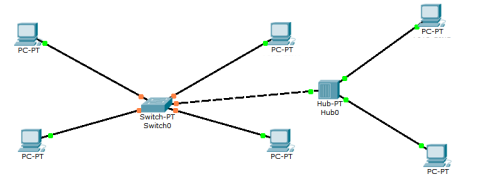
\includegraphics[keepaspectratio,alt={Capture d\textquotesingle écran de Packet Tracer : quatre PC-PT reliés au Switch0 par des traits pleins, un trait pointillé relie le Switch0 au Hub0, deux autres PC-PT sont reliés au Hub0. Les points sont orange côté commutateur (liens en cours de configuration) et verts côté concentrateur et postes.}]{img/reseau-commutateur-concentrateur.png}}

}

\caption{Quatre postes sur un commutateur, relié à un concentrateur qui
porte deux autres postes.}

\end{figure}%

Vous constaterez que vous ne pouvez pas connecter le commutateur au
concentrateur, car il manque un port FastEthernet au commutateur. Vous
allez donc ajouter un port au commutateur :

\begin{enumerate}
\def\labelenumi{\arabic{enumi}.}
\tightlist
\item
  Cliquez sur le commutateur pour ouvrir sa fenêtre de propriétés et
  choisissez l'onglet « Physical » (physique) pour visualiser sa face
  arrière. \textbf{(1)} Éteignez le commutateur en cliquant sur
  l'interrupteur I/O.
\item
  \textbf{(2)} Choisissez dans la liste de gauche un module de type «
  CFE ».
\item
  \textbf{(3)} Faites-le glisser vers un emplacement libre de la face
  arrière du commutateur.
\item
  Rallumez le commutateur, puis fermez la fenêtre. Attendez quelques
  secondes que tout se remette en fonctionnement (connexions vertes).
\end{enumerate}

\begin{figure}[htbp]

{\centering \pandocbounded{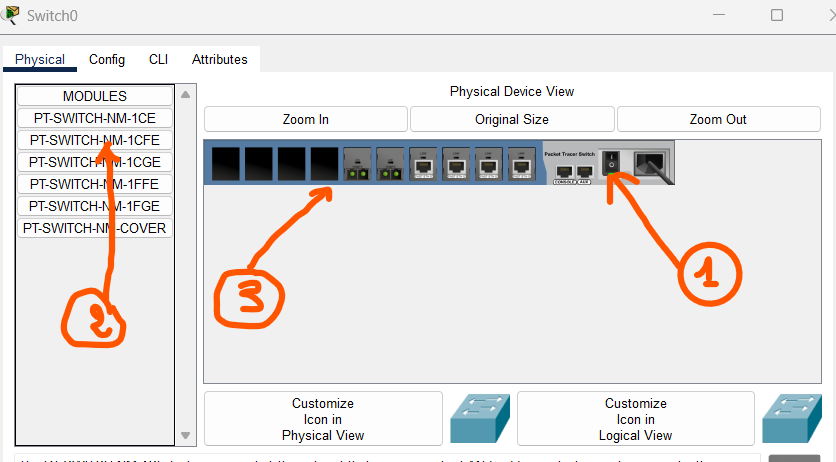
\includegraphics[keepaspectratio,alt={Capture d\textquotesingle écran de la fenêtre Switch0, onglet Physical. La liste de modules à gauche (PT-SWITCH-NM-1CE, 1CFE, 1CGE, 1FFE, 1FGE, COVER) porte la flèche 2 sur le module CFE. La flèche 1 désigne l\textquotesingle interrupteur et la flèche 3 un emplacement libre de la face arrière.}]{img/module-cfe-commutateur.png}}

}

\caption{Face arrière du commutateur : interrupteur (1), module CFE (2)
et emplacement libre (3).}

\end{figure}%

\begin{tcolorbox}[enhanced jigsaw, arc=.35mm, bottomrule=.15mm, bottomtitle=1mm, breakable, colback=white, colbacktitle=quarto-callout-note-color!10!white, colframe=quarto-callout-note-color-frame, coltitle=black, left=2mm, leftrule=.75mm, opacityback=0, opacitybacktitle=0.6, rightrule=.15mm, title=\textcolor{quarto-callout-note-color}{\faInfo}\hspace{0.5em}{Question 5}, titlerule=0mm, toprule=.15mm, toptitle=1mm]

Simulez l'envoi d'un PDU de PC0 vers PC4. Décrivez ce qu'il se passe.

\end{tcolorbox}

\begin{tcolorbox}[enhanced jigsaw, arc=.35mm, bottomrule=.15mm, bottomtitle=1mm, breakable, colback=white, colbacktitle=quarto-callout-note-color!10!white, colframe=quarto-callout-note-color-frame, coltitle=black, left=2mm, leftrule=.75mm, opacityback=0, opacitybacktitle=0.6, rightrule=.15mm, title=\textcolor{quarto-callout-note-color}{\faInfo}\hspace{0.5em}{Question 6}, titlerule=0mm, toprule=.15mm, toptitle=1mm]

Modifiez l'adresse IP de PC5 de telle sorte qu'il ne fasse plus partie
du réseau, puis essayez d'émettre un PDU de PC1 vers PC5. Que se
passe-t-il ?

\end{tcolorbox}

\begin{tcolorbox}[enhanced jigsaw, arc=.35mm, bottomrule=.15mm, bottomtitle=1mm, breakable, colback=white, colbacktitle=quarto-callout-warning-color!10!white, colframe=quarto-callout-warning-color-frame, coltitle=black, left=2mm, leftrule=.75mm, opacityback=0, opacitybacktitle=0.6, rightrule=.15mm, title=\textcolor{quarto-callout-warning-color}{\faExclamationTriangle}\hspace{0.5em}{Avertissement}, titlerule=0mm, toprule=.15mm, toptitle=1mm]

\textbf{ARRÊT : FAIRE VALIDER LE TRAVAIL PAR LE PROFESSEUR AVANT DE
POURSUIVRE}

\end{tcolorbox}

\subsubsection{3. Mise en œuvre d'un
routeur}\label{mise-en-ux153uvre-dun-routeur}

Vous venez de constater que deux ordinateurs ne possédant pas la même
adresse réseau ne peuvent pas communiquer entre eux. Un routeur résout
ce problème.

\begin{tcolorbox}[enhanced jigsaw, arc=.35mm, bottomrule=.15mm, bottomtitle=1mm, breakable, colback=white, colbacktitle=quarto-callout-note-color!10!white, colframe=quarto-callout-note-color-frame, coltitle=black, left=2mm, leftrule=.75mm, opacityback=0, opacitybacktitle=0.6, rightrule=.15mm, title=\textcolor{quarto-callout-note-color}{\faInfo}\hspace{0.5em}{Question 7}, titlerule=0mm, toprule=.15mm, toptitle=1mm]

Modifiez les adresses IP du ou des postes du réseau précédent de façon à
avoir deux réseaux, comme ci-dessous : PC0 à PC3 dans le réseau 1, PC4
et PC5 dans le réseau 2.

\end{tcolorbox}

\begin{figure}[htbp]

{\centering \pandocbounded{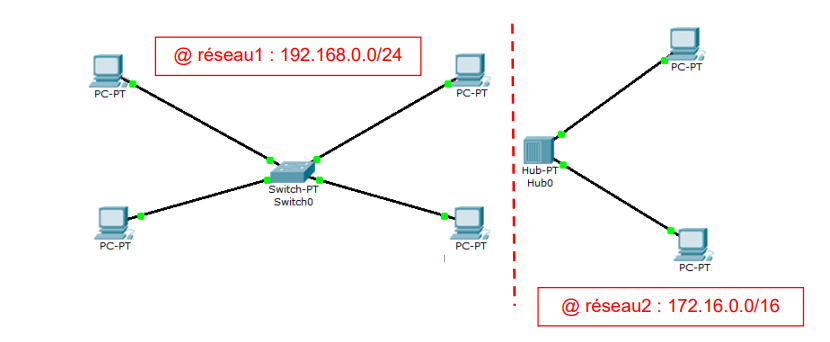
\includegraphics[keepaspectratio,alt={Schéma de Packet Tracer : à gauche, quatre PC-PT reliés au Switch0, avec l\textquotesingle étiquette « adresse réseau 1 : 192.168.0.0/24 ». À droite, séparés par un trait pointillé vertical, deux PC-PT reliés au Hub0, avec l\textquotesingle étiquette « adresse réseau 2 : 172.16.0.0/16 ».}]{img/deux-reseaux-routeur.png}}

}

\caption{Réseau 1 (commutateur et quatre postes) et réseau 2
(concentrateur et deux postes), séparés par un trait pointillé.}

\end{figure}%

Supprimez d'abord le câble qui relie le commutateur au concentrateur :
les deux réseaux ne doivent plus avoir aucun lien physique entre eux.

Ajoutez ensuite un routeur entre les deux réseaux (choisissez le routeur
« 1941 » ou « 2941 »). Connectez le routeur aux deux réseaux différents,
via le hub et via le switch.

\begin{tcolorbox}[enhanced jigsaw, arc=.35mm, bottomrule=.15mm, bottomtitle=1mm, breakable, colback=white, colbacktitle=quarto-callout-note-color!10!white, colframe=quarto-callout-note-color-frame, coltitle=black, left=2mm, leftrule=.75mm, opacityback=0, opacitybacktitle=0.6, rightrule=.15mm, title=\textcolor{quarto-callout-note-color}{\faInfo}\hspace{0.5em}{Question 8}, titlerule=0mm, toprule=.15mm, toptitle=1mm]

Quel type de câble est utilisé pour relier un hub ou un switch à un
routeur ?

\end{tcolorbox}

Vous observez que les deux connexions sont de couleur rouge : la
communication entre les deux réseaux ne fonctionne pas dans l'état
actuel. En déplaçant le curseur sur le routeur, vous pouvez lire dans la
fenêtre d'information « Link Down » (ou « Liaison Bas »). Les interfaces
ne sont donc pas opérationnelles.

Il faut configurer le routeur en lui attribuant deux adresses IP
appartenant respectivement aux deux réseaux à interconnecter. Pour cela
:

\begin{enumerate}
\def\labelenumi{\arabic{enumi}.}
\tightlist
\item
  Cliquez sur le routeur pour ouvrir la fenêtre de propriétés.
\item
  Sélectionnez l'onglet « Config ».
\item
  Dans le menu de gauche, cliquez sur « INTERFACE \textgreater{}
  GigabitEthernet0/0 ».
\item
  Saisissez une adresse IP disponible et le masque de sous-réseau
  correspondant au premier réseau.
\item
  Cochez la case pour activer le port (Port Status : On).
\item
  Répétez la même procédure pour l'interface « GigabitEthernet0/1 »,
  avec une adresse IP et le masque appropriés pour le second réseau.
\end{enumerate}

Cette configuration permet au routeur de faire le lien entre les deux
réseaux. Les connexions passent du rouge au vert.

\begin{tcolorbox}[enhanced jigsaw, arc=.35mm, bottomrule=.15mm, bottomtitle=1mm, breakable, colback=white, colbacktitle=quarto-callout-note-color!10!white, colframe=quarto-callout-note-color-frame, coltitle=black, left=2mm, leftrule=.75mm, opacityback=0, opacitybacktitle=0.6, rightrule=.15mm, title=\textcolor{quarto-callout-note-color}{\faInfo}\hspace{0.5em}{Question 9}, titlerule=0mm, toprule=.15mm, toptitle=1mm]

Simulez l'envoi d'un PDU entre PC0 et PC4. L'essai est-il concluant ?

\end{tcolorbox}

Cela ne fonctionne toujours pas. PC4 n'est pas joignable, car PC0
n'appartient pas au même réseau. Il faut indiquer à PC0 qu'il peut le
joindre en passant par le routeur.

Lorsqu'un poste envoie des données à un hôte qui n'est pas sur son
réseau, il doit les envoyer à un routeur. C'est seulement ensuite que le
routeur se charge d'acheminer (router) les données sur l'autre réseau.
Cliquez sur PC0, onglet « Desktop », puis « IP Configuration ». Entrez
dans « Default Gateway » (ou « Passerelle ») l'adresse IP de l'interface
du routeur située sur le réseau de PC0.

\begin{tcolorbox}[enhanced jigsaw, arc=.35mm, bottomrule=.15mm, bottomtitle=1mm, breakable, colback=white, colbacktitle=quarto-callout-note-color!10!white, colframe=quarto-callout-note-color-frame, coltitle=black, left=2mm, leftrule=.75mm, opacityback=0, opacitybacktitle=0.6, rightrule=.15mm, title=\textcolor{quarto-callout-note-color}{\faInfo}\hspace{0.5em}{Question 10}, titlerule=0mm, toprule=.15mm, toptitle=1mm]

Simulez à nouveau l'envoi d'un PDU entre PC0 et PC4. L'essai est-il
concluant ? Observez où le PDU est transmis, puis où il s'arrête.
Pourquoi PC4 ne peut-il pas répondre à PC0 ?

\end{tcolorbox}

\begin{tcolorbox}[enhanced jigsaw, arc=.35mm, bottomrule=.15mm, bottomtitle=1mm, breakable, colback=white, colbacktitle=quarto-callout-note-color!10!white, colframe=quarto-callout-note-color-frame, coltitle=black, left=2mm, leftrule=.75mm, opacityback=0, opacitybacktitle=0.6, rightrule=.15mm, title=\textcolor{quarto-callout-note-color}{\faInfo}\hspace{0.5em}{Question 11}, titlerule=0mm, toprule=.15mm, toptitle=1mm]

Indiquez la passerelle pour PC4. Simulez à nouveau l'envoi d'un PDU
entre PC0 et PC4. L'essai est-il concluant ? Décrivez le trajet de
l'aller et celui du retour.

\end{tcolorbox}

\begin{tcolorbox}[enhanced jigsaw, arc=.35mm, bottomrule=.15mm, bottomtitle=1mm, breakable, colback=white, colbacktitle=quarto-callout-note-color!10!white, colframe=quarto-callout-note-color-frame, coltitle=black, left=2mm, leftrule=.75mm, opacityback=0, opacitybacktitle=0.6, rightrule=.15mm, title=\textcolor{quarto-callout-note-color}{\faInfo}\hspace{0.5em}{Question 12}, titlerule=0mm, toprule=.15mm, toptitle=1mm]

Modifiez la configuration des autres hôtes de manière à ce que tous les
postes puissent communiquer entre eux. Vérifiez le fonctionnement.

\end{tcolorbox}

\subsection{Vérification et compte
rendu}\label{vuxe9rification-et-compte-rendu}

Avant de demander la validation, vérifiez que :

\begin{itemize}
\tightlist
\item
  les liens du commutateur, du concentrateur et du routeur affichent
  tous un point vert ;
\item
  un PDU envoyé de n'importe quel poste vers n'importe quel autre poste
  est acquitté (marque verte dans la liste des événements) ;
\item
  chaque poste a une adresse IP, un masque et une passerelle cohérents
  avec son réseau.
\end{itemize}

Livrables : vos réponses aux questions 1 à 13 et votre fichier Packet
Tracer enregistré.

\subsection{Synthèse}\label{synthuxe8se}

\begin{tcolorbox}[enhanced jigsaw, arc=.35mm, bottomrule=.15mm, bottomtitle=1mm, breakable, colback=white, colbacktitle=quarto-callout-note-color!10!white, colframe=quarto-callout-note-color-frame, coltitle=black, left=2mm, leftrule=.75mm, opacityback=0, opacitybacktitle=0.6, rightrule=.15mm, title=\textcolor{quarto-callout-note-color}{\faInfo}\hspace{0.5em}{Question 13}, titlerule=0mm, toprule=.15mm, toptitle=1mm]

Conclusions sur les observations effectuées. Expliquez comment un hôte
sur un réseau peut communiquer avec un hôte d'un réseau différent. Que
doit-on faire pour configurer un routeur ? Qu'est-ce qu'une « passerelle
» ?

\end{tcolorbox}

\begin{tcolorbox}[enhanced jigsaw, arc=.35mm, bottomrule=.15mm, bottomtitle=1mm, breakable, colback=white, colbacktitle=quarto-callout-warning-color!10!white, colframe=quarto-callout-warning-color-frame, coltitle=black, left=2mm, leftrule=.75mm, opacityback=0, opacitybacktitle=0.6, rightrule=.15mm, title=\textcolor{quarto-callout-warning-color}{\faExclamationTriangle}\hspace{0.5em}{Avertissement}, titlerule=0mm, toprule=.15mm, toptitle=1mm]

\textbf{ARRÊT : FAIRE VALIDER LE TRAVAIL PAR LE PROFESSEUR AVANT DE
POURSUIVRE}

\end{tcolorbox}

La suite se trouve dans la \href{../tp-creation-lan-3/index.qmd}{partie
3 : réseau sans fil et cahier des charges}.

\subsection{Pour aller plus loin}\label{pour-aller-plus-loin}

\begin{itemize}
\tightlist
\item
  Documentation de Cisco Packet Tracer (Cisco Networking Academy) :
  \url{https://www.netacad.com/cisco-packet-tracer}
\item
  RFC 1812, \emph{Requirements for IP Version 4 Routers} :
  \url{https://www.rfc-editor.org/rfc/rfc1812}
\end{itemize}




\end{document}
